\documentclass[11pt]{article}
\usepackage{cse216,hyperref}
% use the tikz package to draw automata
\usepackage{tikz}
\usetikzlibrary{arrows,positioning,automata}
\def\title{HW 7}
\begin{document}
\maketitle

\section*{Due November 24 at 3:00 pm}

\textbf{(2 questions, 55 points total)}

\begin{qunlist}

  \q{30}{Synthesis Games}\\
  Consider the following 2-player graph game:

  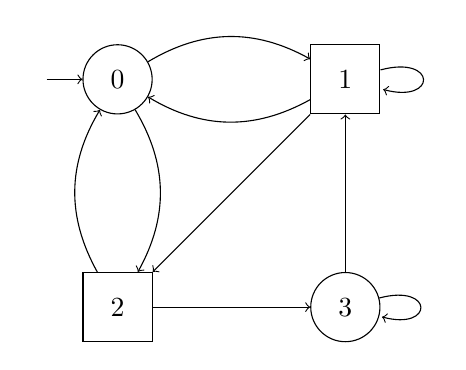
\begin{tikzpicture}[node distance=2cm]
    \node[state, initial, initial text=, align=center] (s0) {0};
    \node[state, rectangle, right= of s0, align=center] (s1) {1};
    \node[state, rectangle, below= of s0, align=center] (s2) {2};
    \node[state, right= of s2, align=center] (s3) {3};

    \path[->]
    (s0) edge[bend left] (s1)
    (s0) edge[bend left] (s2)
    (s1) edge[bend left] (s0)
    (s1) edge[loop right] (s1)
    (s1) edge (s2)
    (s2) edge[bend left] (s0)
    (s2) edge (s3)
    (s3) edge (s1)
    (s3) edge[loop right] (s3);
  \end{tikzpicture}

  \begin{qparts}
  \item
    What is the controllable predecessor of the set $\{1\}$?

    \begin{answer}

      \begin{itemize}
        \item State 0 has edge $0 \to 1$, so it is included.
        \item State 3 has edge $3 \to 1$, so it is included.
        \item State 1 successors $\{0,1,2\} \not\subseteq \{1\}$, so it is not included.
        \item State 2 successors $\{0,3\} \not\subseteq \{1\}$, so it is not included.
      \end{itemize}
      So the pred of 1 is $\{0, 3\}$.
    \end{answer}

  \item
    Continue using the fixed-point reachability game algorithm to find all states from which player 1 (the circle player) has a winning strategy to reach state 1.

    \begin{answer}
      Iterate $W_{i+1} = W_i \cup pred(W_i)$ starting from $W_0 = \{1\}$:
      \begin{itemize}
        \item $W_1 = \{1\} \cup \{0,3\} = \{0,1,3\}$.
        \item $W_2 = W_1 \cup pred(W_1)$. State 2 (square) has successors $\{0,3\} \subseteq W_1$, so it is added. Thus $W_2 = \{0,1,2,3\}$.
        \item $W_3 = W_2$, so the fixed point is reached.
      \end{itemize}
      Player 1 wins the reachability game from every state $\{0,1,2,3\}$, for example with the strategy: from 0 move to 1, from 3 move to 1. (From 2, either move player 2 makes lands in 0 or 3.)
    \end{answer}

  \item
    What is the controllable predecessor of the set $\{0, 3\}$?

    \begin{answer}
      \begin{itemize}
        \item State 0 successors $\{1,2\}$, neither in $\{0,3\}$, so it is not included.
        \item State 3 has the self-loop $3 \to 3$, so it is included.
        \item State 1 successors $\{0,1,2\} \not\subseteq \{0,3\}$, so it is not included.
        \item State 2 successors $\{0,3\} \subseteq \{0,3\}$, so it is included.
      \end{itemize}
      So $pred(\{0,3\}) = \{2, 3\}$.
    \end{answer}

  \item
    Does player 1 have a winning strategy for the B\"uchi objective with $G = \{0, 3\}$?
    If so, give a winning strategy for player 1; otherwise give a winning strategy for player 2 (that causes player 1 to lose).

    (\emph{N.B.} You don't need to use the B\"uchi game algorithm if you'd rather just eyeball the solution.)

    \begin{answer}
      Yes, from the initial state 0. A winning (memoryless) strategy for player 1 is:
      \begin{itemize}
        \item at state 0, move to state 2;
        \item at state 3, take the self-loop to state 3.
      \end{itemize}
      Under this strategy, state 1 is never entered. From state 2, player 2 must move to either 0 or 3, both of which are in $G$. If play goes to 0, player 1 goes back to 2, so $G$ is visited at least every two steps. If play goes to 3, it stays at 3 forever. In every case $G$ is visited infinitely often.

    \end{answer}
  \end{qparts}

  \q{25}{Verification using Inductive Invariants}\\
  Consider the following program, where \texttt{x} and \texttt{y} are integers (no overflow, for simplicity):
\begin{verbatim}
assume x > 0
y = 1
while y < x:
  y = 2 * y
assert x <= y and y <= 2 * x
\end{verbatim}

  \begin{qparts}
  \item
    What is a suitable invariant $\varphi(x,y)$ to use to prove the assertion?

    \begin{answer}
      \[
        \varphi(x,y) \;:=\; y \le 2x .
      \]
    \end{answer}

  \item
    Write SMT formulas for the two conditions $\varphi$ must satisfy to be an inductive invariant.
    (If your invariant is correct, these formulas should be valid.)

    \begin{answer}
      Initiation
      \begin{equation}\label{eq:initiation}
        \forall x, y \in \mathbb{Z}.\; \bigl(x > 0 \wedge y = 1\bigr) \rightarrow y \le 2x
      \end{equation}
      Consecution (one loop iteration preserves the invariant), with $y'$ the value of $y$ after the loop body:
      \begin{equation}\label{eq:consecution}
        \forall x, y, y' \in \mathbb{Z}.\; \bigl(y \le 2x \wedge y < x \wedge y' = 2y\bigr) \rightarrow y' \le 2x
      \end{equation}
      Both are valid. For \eqref{eq:initiation}, $x \ge 1$ over the integers gives $2x \ge 2 > 1$. For \eqref{eq:consecution}, $y < x$ gives $y' = 2y < 2x$.
    \end{answer}

  \item
    Write an SMT formula for the final condition you need to check to see whether the assertion follows from the invariant and the fact that the loop has terminated.
    (If your invariant is correct, this formula should be valid.)

    \begin{answer}
      \begin{equation}\label{eq:exit}
        \forall x, y \in \mathbb{Z}.\; \bigl(y \le 2x \wedge \neg (y < x)\bigr) \rightarrow \bigl(x \le y \wedge y \le 2x\bigr)
      \end{equation}
      This is valid: $\neg(y < x)$ is exactly $x \le y$, and $y \le 2x$ is the invariant.
      (To check any of \eqref{eq:initiation}--\eqref{eq:exit} with an SMT solver, assert the negation of the body and check that the result is \texttt{unsat}.)
    \end{answer}

  \end{qparts}

\end{qunlist}
\end{document}
